\documentclass[letterpaper,11pt]{article}

% Soporte para los acentos.
\usepackage[utf8]{inputenc}
\usepackage[T1]{fontenc}    
% Idioma español.
\usepackage[spanish,mexico, es-tabla]{babel}
% Soporte de símbolos adicionales (matemáticas)
\usepackage{multirow}
\usepackage{amsmath}		
\usepackage{amssymb}		
\usepackage{amsthm}
\usepackage{amsfonts}
\usepackage{latexsym}
\usepackage{enumerate}
\usepackage{ragged2e}
\usepackage{graphicx}
% Modificamos los márgenes del documento.
\usepackage[lmargin=2cm,rmargin=2cm,top=2cm,bottom=2cm]{geometry}

\title{Facultad de Ciencias, UNAM \\ 
       Reconocimiento de patrones y aprendizaje automatizado \\ 
       Tarea 1}
\author{Rubí Rojas Tania Michelle}
\date{\today}

\begin{document}
\maketitle

\begin{enumerate}
    % Ejercicio 1.
    \item Considera la siguiente expresión para calcular los elementos de un 
    conjunto de punto flotante 
    \begin{equation*}
        2(\beta - 1) \beta^{p-1} (L - l + 1) + 1
    \end{equation*}

    donde $\beta$ es la base, $L$ es el exponente más grande y $l$ el más 
    pequeño. Calcula todos los elementos para los siguientes valores 
    $\beta = 2$, $L = 2$ y $l = -1$, donde los números tienen $3$ cifras 
    significativas.

    Construye todos los números de este conjunto F.

    \textsc{Solución:} Tenemos un total de 
    \begin{align*}
        2(\beta - 1) \beta^{p-1} (L - l + 1) + 1
        &= 2(2 - 1) 2^{3-1} (2 - (-1) + 1) + 1 \\ 
        &= 2(1) 2^{2} (4) + 1 \\ 
        &= 8 (4) + 1 \\ 
        &= 33
    \end{align*}

    números de punto flotante en este sistema (incluyendo el cero). Por otro 
    lado, sabemos que si $x \in F$ entonces su opuesto $-x \in F$. Además, 
    tenemos que el conjunto $F$ está acotado superior e inferiormente por 
    \begin{equation*}
        x_{\text{min}} = \beta^{l-1} = 2^{-1-1} = 2^{-2} = \frac{1}{4}
    \end{equation*}
    \begin{equation*}
        x_{\text{max}} 
        = \beta^L (1 - \beta^{-p}) 
        = 2^2 (1 - 2^{-3})
        = \frac{7}{2}
    \end{equation*}

    Es decir, $x_{\text{min}} = \frac{1}{4}$ es el menor número representable 
    en el sistema; mientras que $x_{\text{max}} = \frac{7}{2}$ es el máximo 
    número representable en el conjunto.

    Como los elementos del conjunto $F$, diferentes de cero, son de la forma 
    $\pm (.a_1 a_2 a_3)_2 \cdot 2^e$ donde 
    \begin{itemize}
        \item $a_1 = 1$
        \item $a_2, a_3 = 0, 1$
        \item $e = -1, 0, 1, 2$
    \end{itemize}

    entonces las distintas fracciones positivas son: 
    \begin{equation*}
        (.100)_2 
        = \frac{1}{2} + \frac{0}{2^2} + \frac{0}{2^3}
        = \frac{1}{2} \quad \quad \quad
        (.101)_2
        = \frac{1}{2} + \frac{0}{2^2} + \frac{1}{2^3}
        = \frac{5}{8}
    \end{equation*}
    \begin{equation*}
        (.110)_2
        = \frac{1}{2} + \frac{1}{2^2} + \frac{0}{2^3}
        = \frac{3}{4} \quad  \quad \quad 
        (.111)_2
        = \frac{1}{2} + \frac{1}{2^2} + \frac{1}{2^3}
        = \frac{7}{8}
    \end{equation*}

    Combinando estas mantisas con los exponentes obtenemos $16$ de los 
    $33$ números del conjunto $F$, los cuales corresponden a sus números 
    positivos:
    \begin{align*}
        (.100)_2 &\cdot 2^{-1} = \frac{1}{2} \cdot \frac{1}{2} = 
        \frac{1}{4} 
        & (.100)_2 &\cdot 2^0 = \frac{1}{2} \cdot 1 = \frac{1}{2}              
        &  (.100)_2 &\cdot 2^1 = \frac{1}{2} \cdot 2 = 1 \\
        (.100)_2 &\cdot 2^2 = \frac{1}{2} \cdot 4 = 2 
        & (.101)_2 &\cdot 2^{-1} = \frac{5}{8} \cdot \frac{1}{2} = 
        \frac{5}{16}  
        & (.101)_2 &\cdot 2^0 = \frac{5}{8} \cdot 1 = \frac{5}{8} \\
        (.101)_2 &\cdot 2^1 = \frac{5}{8} \cdot 2 = \frac{5}{4}
        & (.101)_2 &\cdot 2^2 = \frac{5}{8} \cdot 4 = \frac{5}{2} 
        & (.110)_2 &\cdot 2^{-1} = \frac{3}{4} \cdot \frac{1}{2} = 
        \frac{3}{8} \\
        (.110)_2 &\cdot 2^0 = \frac{3}{4} \cdot 1 = \frac{3}{4} 
        & (.110)_2 &\cdot 2^1 = \frac{3}{4} \cdot 2 = \frac{3}{2} 
        & (.110)_2 &\cdot 2^2 = \frac{3}{4} \cdot 4 = 3 \\
        (.111)_2 &\cdot 2^{-1} = \frac{7}{8} \cdot \frac{1}{2} 
        = \frac{7}{16} 
        & (.111)_2 &\cdot 2^0 = \frac{7}{8} \cdot 1 = \frac{7}{8} 
        & (.111)_2 &\cdot 2^1 = \frac{7}{8} \cdot 2 = \frac{7}{4} \\ 
        (.111)_2 &\cdot 2^2 = \frac{7}{8} \cdot 4 = \frac{7}{2}
    \end{align*}

    Por lo tanto, los $33$ números del conjunto $F$ son:
    \begin{equation*}
        0, \pm \frac{1}{4}, \pm \frac{1}{2}, \pm 1, \pm 2, \pm \frac{5}{16},
        \pm \frac{5}{8}, \pm \frac{5}{4}, \pm \frac{5}{2}, \pm \frac{3}{8}, 
        \pm \frac{3}{4}, \pm \frac{3}{2}, \pm 3, \pm \frac{7}{16}, 
        \pm \frac{7}{8}, \pm \frac{7}{4}, \pm \frac{7}{2}
    \end{equation*}
    
    % Ejercicio 2.
    \item Determina el condicionamiento de la siguiente función:
    \begin{equation*}
        f(x) = \sqrt{x - 1} - \sqrt{x}
    \end{equation*}

    \textsc{Solución:} Primero, calculamos la derivada de la función $f(x)$.
    \begin{equation*}
        f'(x) 
        = \frac{d}{dx} (\sqrt{x - 1} - \sqrt{x}) 
        = \frac{d}{dx} (\sqrt{x - 1}) - \frac{d}{dx} (\sqrt{x}) 
        = \frac{1}{2 \sqrt{x - 1}} - \frac{1}{2 \sqrt{x}} 
    \end{equation*}

    El número de condición de la función $f(x)$ está determinada por 
    \begin{equation*}
        C(x) = \left| \frac{x f'(x)}{f(x)} \right|
    \end{equation*}

    Por lo que, 
    \begin{align*}
        C(x) &= \left| \frac{x \left(\frac{1}{2 \sqrt{x - 1}} - 
                                     \frac{1}{2 \sqrt{x}}\right)}
                            {\sqrt{x - 1} - \sqrt{x}} \right| \\ 
             &= \left| \frac{x \left(\frac{1}{2} 
                                     \left(\frac{1}{\sqrt{x - 1}} - 
                                           \frac{1}{\sqrt{x}}\right) \right)}
                            {\sqrt{x - 1} - \sqrt{x}} \right| \\ 
             &= \left| \frac{x}{2} \frac{\left(\frac{\sqrt{x} - \sqrt{x-1}}
                                                    {\sqrt{x-1} \sqrt{x}}\right)}
                            {\sqrt{x - 1} - \sqrt{x}} \right| \\ 
             &= \left| \frac{x}{2} \left(- \frac{1}
                                                {\sqrt{x - 1} \sqrt{x}}\right) \right| \\ 
             &= \left|- \frac{x}{2 \sqrt{x - 1} \sqrt{x}} \right| \\ 
             &= \frac{x}{2 \sqrt{x - 1} \sqrt{x}} 
    \end{align*}

    Por lo tanto, el número de condición de la función 
    $f(x) = \sqrt{x - 1} - \sqrt{x}$ es $\frac{x}{2 \sqrt{x - 1} \sqrt{x}}$. 

    % Ejercicio 3.
    \item Implementa los algoritmos de la bisección y de newton en un 
    script. Muestra su funcionamiento con la siguiente función 
    \begin{equation*}
        g(x) = x^3 - x - 1
    \end{equation*}

    \textsc{Solución:} El algoritmo de \texttt{biseccion} fue implementado de 
    la siguiente manera
    \begin{center}
        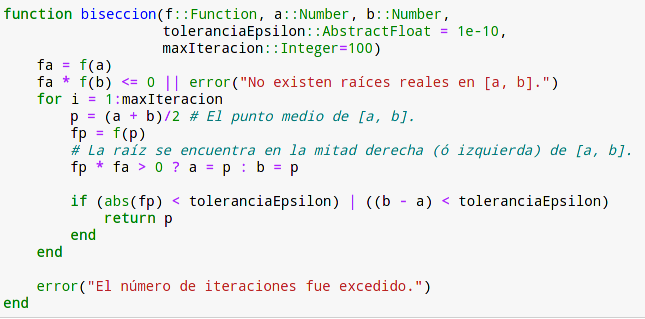
\includegraphics[width=0.6\textwidth]{imagenes/biseccion.png}
    \end{center}

    Mostramos su funcionamiento con la función $g(x) = x^3 - x - 1$.
    \begin{center}
        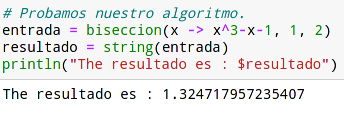
\includegraphics[width=0.35\textwidth]{./imagenes/biseccion_funcionamiento.png}
    \end{center}

    Por otro lado, el algoritmo de \texttt{newton} fue implementado de la 
    siguiente manera
    \begin{center}
        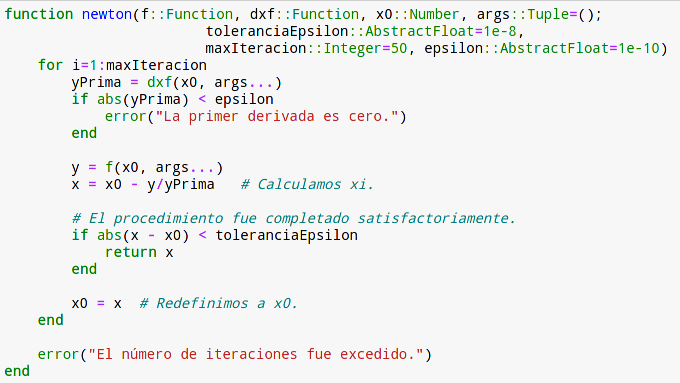
\includegraphics[width=0.6\textwidth]{imagenes/newton.png}
    \end{center}

    Mostramos su funcionamiento con la función $g(x) = x^3 - x - 1$.
    \begin{center}
        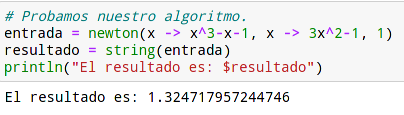
\includegraphics[width=0.4\textwidth]{./imagenes/newton_funcionamiento.png}
    \end{center}

    % Ejercicio 4.
    \item Usa los métodos implementados en la pregunta $3$ para encontrar $x^*$
    que soluciona $g(x^*) = 0$ y $h(x^*) = 0$ en las siguientes funciones
    \begin{equation*}
        g(x) = cos(x) - x
    \end{equation*}

    en el intervalo $[\frac{1}{2}, 1]$, y 
    \begin{equation*}
        h(x) = x^2 - x - 1
    \end{equation*}

    en el intervalo $[1, 2]$. En este caso, la tolerancia debe ser mínimo de 
    $10^{-8}$.

    \textsc{Solución:} Usándo le método de la \texttt{biseccion} obtenemos que 
    el valor $x^*$ que soluciona 
    \begin{itemize}
        \item $g(x) = cos(x) - x$ es $0.7390$.
        \begin{center}
            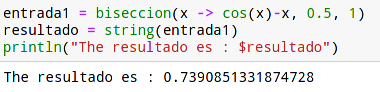
\includegraphics[width=0.4\textwidth]{imagenes/biseccion_g(x).png}
        \end{center}

        \item $h(x) = x^2 - x - 1$ es $1.6180$.
        \begin{center}
            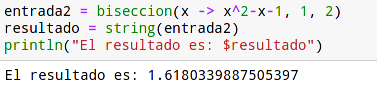
\includegraphics[width=0.4\textwidth]{imagenes/biseccion_h(x).png}
        \end{center}
    \end{itemize}

    Comprobamos los resultados obtenidos con el método de \texttt{newton}, de 
    tal forma que el valor $x^*$ que soluciona 
    \begin{itemize}
        \item $g(x) = cos(x) - x$ es $0.7390$
        \begin{center}
            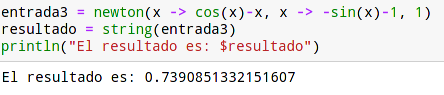
\includegraphics[width=0.45\textwidth]{imagenes/newton_g(x).png}
        \end{center}

        \item $h(x) = x^2 - x - 1$ es $1.6180$
        \begin{center}
            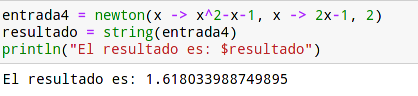
\includegraphics[width=0.45\textwidth]{imagenes/newton_h(x).png}
        \end{center}
    \end{itemize}
    
    \newpage
    % Ejercicio 5.
    \item Muestra que el polinomio característico $p(\lambda)$ de una matriz 
    $A \in \mathcal{R}^{2 \times 2}$ se puede expresar como 
    \begin{equation*}
        p(\lambda) = \lambda^2 - \lambda tr(A) + det(A)
    \end{equation*}

    donde tr(A) es la traza de la matriz $A$ y det(A) es el determinante de la 
    misma. 

    \begin{proof}
        Sea $A = \begin{pmatrix} a & b \\ c & d \\ \end{pmatrix} \in 
        M_{2 \times 2}(R)$. Entonces, tenemos que
        \begin{align*}
            p(\lambda) 
            &= det(A - \lambda I_n)
            && \text{definición de $p(\lambda)$} \\
            &= det \left( \begin{pmatrix} a & b \\ c & d \end{pmatrix} - 
                          \lambda \begin{pmatrix} 1 & 0 \\ 0 & 1 \end{pmatrix}
                   \right) 
            && \text{multiplicación escalar de matrices} \\
            &= det \left(\begin{pmatrix} a & b \\ c & d \\ \end{pmatrix} - 
                         \begin{pmatrix} \lambda & 0 \\ 0 & \lambda \end{pmatrix} 
                   \right)
            && \text{sustituyendo valores} \\
            &= det \left( \begin{pmatrix} a - \lambda & b \\ c & d -\lambda 
                          \end{pmatrix} \right)
            && \text{resta de matrices} \\
            &= (a - \lambda) (d - \lambda) - bc
            && \text{definición del determinante} \\ 
            &= ad - a\lambda - d\lambda + \lambda^2 - bc
            && \text{álgebra} \\
            &= ad - (a + d)\lambda + \lambda^2 - bc
            && \text{factorizando} \\
            &= \lambda^2 - (a + d)\lambda + (ad - bc)
            && \text{reacomodando la expresión} \\
            &= \lambda^2 - tr(A)\lambda + det(A)
            && \text{definición de tr(A) y det(A)} \\
            &= \lambda^2 - \lambda tr(A) + det(A) 
            && \text{conmutatividad de la multiplicación}
        \end{align*}

        Por lo tanto, el polinomio característico de la matriz $A$ puede ser 
        expresado como 
        \begin{equation*}
            p(\lambda) = \lambda^2 - \lambda tr(A) + det(A)
        \end{equation*}
    \end{proof}

    % Ejercicio 6.
    \item Utiliza el algoritmo de KNN con el dataset \texttt{"trees.csv"}. Este 
    dataset cuenta con tres variables o atributos: el diámetro a la altura del 
    pecho, la altura y el volumen de varios árboles. Utilizándo los notebooks 
    provistos en clase, responde:
    \begin{enumerate}
        % Ejercicio 6.a
        \item Define dos variables independientes y una dependiente. Justifica 
        tu elección.

        \textsc{Solución:} Definimos a las variables \texttt{"Girth"} y 
        \texttt{"Height"} como independientes y a la variable \texttt{"Volume"}
        como dependiente. La elección la realizamos de esta forma porque es 
        más sencillo medir la altura y el diámetro a la altura del pecho, que 
        medir el volúmen de los árboles (estuve leyendo un poco al respecto, y 
        para calcular el volumen sin necesidad de talar el árbol se necesitan 
        algunas técnicas complicadas y muy tardadas). Por lo que, es útil poder 
        predecir el volumen del árbol a partir de la altura y el diámetro dados.

        % Ejercicio 6.b
        \item Normaliza las variables, ¿para qué hacemos esto?

        \textsc{Solución:} Para que funcionen mejor muchos algoritmos de 
        \textit{Machine Learning} hay que normalizar las variables de entrada 
        al algoritmo. Normalizar significa, en este caso, comprimir o extender 
        los valores de la variable para que estén en un rango definido.

        El escalador \textbf{MinMaxScaler} transforma las características 
        escalándolas a un rango dado, por defecto $(0, 1)$, aunque puede ser 
        personalizado. Este tipo de escalado suele denominarse frecuentemente 
        como \textit{normalización} de datos.
        \begin{center}
            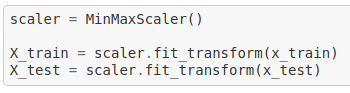
\includegraphics[width=0.4\textwidth]{imagenes/norma.png}
        \end{center}

        % Ejercicio 6.c
        \item Separa tu dataset en conjunto de entrenamiento y conjunto de 
        prueba. ¿Por qué hacemos esto?

        \textsc{Solución:} Una vez que seleccionamos el mejor modelo que se 
        puede crear con los datos disponibles, se tiene que comprobar su 
        capacidad prediciéndo nuevas observaciones que no se hayan empleado 
        para entrenarlo, de esta forma se verifica si el modelo se puede 
        generalizar. Una estrategia para hacer esto es dividir (de manera 
        aleatoria, o no) los datos en dos grupos, ajustar el modelo con el 
        primer grupo y estimar la precisión de las predicciones con el 
        segundo conjunto.

        El tamaño adecuado para las particiones depende de la cantidad de 
        datos disponibles y la seguridad que se necesite en la estimación 
        del error, pero en general dividir el conjunto en un $80-20$ 
        (entrenamiento - prueba) suele dar buenos resultados.
        \begin{center}
            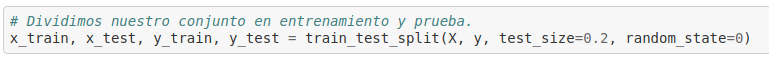
\includegraphics[width=0.8\textwidth]{imagenes/train.png}
        \end{center}

        En este caso, utilizamos la función \texttt{train\_test\_split} para 
        poder dividir nuestro conjunto de datos en entrenamiento y prueba con 
        los porcentajes mencionamos anteriormente. 

        % Ejercicio 6.d
        \item Encuentra la $k$ óptima para aplicar el algoritmo.
        
        \textsc{Solución:} Para elegir el valor óptimo de $k$ podemos utilizar 
        la tasa de error obtenida sobre el conjunto de prueba, para así elegir 
        aquella donde encontremos el valor más pequeño. Para lograr esto, 
        aplicaremos el algoritmo probando varios valores de $k$ y en función de 
        ello determinaremos aquella que minimice el error en el conjunto de 
        prueba.
        \begin{center}
            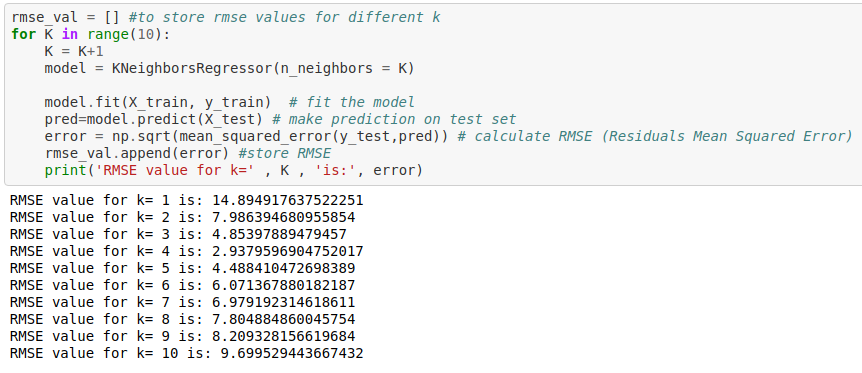
\includegraphics[width=0.8\textwidth]{imagenes/k_value.png}
        \end{center}

        Graficamos los valores obtenidos.
        \begin{center}
            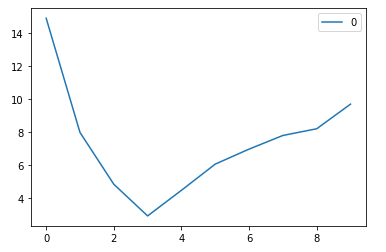
\includegraphics[width=0.4\textwidth]{imagenes/k_grafica.png}
        \end{center}

        De esta forma, podemos notar que el valor $k=3$ es el que minimiza el
        error en el conjunto de prueba, así que aplicaremos el algoritmo con 
        este valor de $k$.
        \begin{center}
            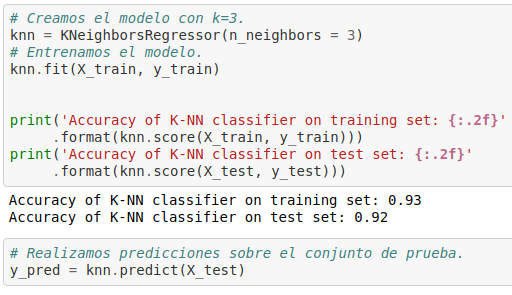
\includegraphics[width=0.5\textwidth]{imagenes/k_modelo.png}
        \end{center}

        Comparamos los resultados de las predicciones con sus valores 
        originales.
        \begin{center}
            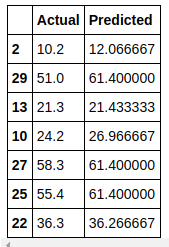
\includegraphics[width=0.2\textwidth]{imagenes/k_predicciones.png}
        \end{center}

        % Ejercicio 6.e
        \item Obtén el MSE del modelo calibrado aplicado al conjunto de prueba.
        
        \textsc{Solución:} Para este modelo obtenemos un $MSE$ con valor de 
        $23.56$.
        \begin{center}
            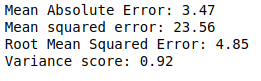
\includegraphics[width=0.4\textwidth]{imagenes/k_mse.png}
        \end{center}
    \end{enumerate}

    % Ejercicio 7.
    \item Utiliza el método de regresión lineal, o en otras palabras, ajusta 
    un modelo lineal a las observaciones del dataset \texttt{"trees.csv"}. 
    Utiliza la misma definición de variables independientes y dependientes del 
    ejercicio anterior, así como el mismo conjunto de entrenamiento y de prueba.
    Responde:
    \begin{enumerate}
        % Ejercicio 7.a
        \item ¿Cuál es el MSE del modelo lineal que construiste?
        
        \textsc{Solución:} Construimos la regresión múltiple tomando a las 
        variables \texttt{Girth, Height} como independientes y a la variable 
        \texttt{Volume} como dependiente. 

        Separamos nuestro conjunto de datos en entrenamiento y prueba, como 
        lo hicimos anteriormente.
        \begin{center}
            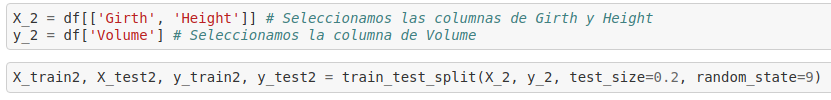
\includegraphics[width=0.75\textwidth]{imagenes/train_lineal.png}
        \end{center}

        \newpage
        Construimos el modelo.
        \begin{center}
            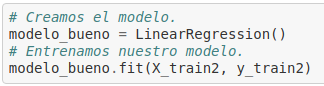
\includegraphics[width=0.4\textwidth]{imagenes/modelo_lineal.png}
        \end{center}

        Visualizamos los coeficientes obtenidos del modelo.
        \begin{center}
            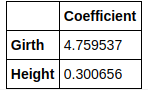
\includegraphics[width=0.2\textwidth]{imagenes/coef.png}
        \end{center}

        Esto significa que cuando la variable \texttt{Girth} incrementa en una 
        unidad (pulgada), entonces \texttt{Volume} incrementa en $4.75$ 
        unidades (pies cúbicos). De manera análoga, cuando \texttt{Height} 
        incrementa en una unidad, entonces \texttt{Volume} incrementa en 
        $0.3$ pies cúbicos. Esto suponiéndo que la otra variable independiente
        no cambia.

        Luego, realizamos predicciones sobre el conjunto de prueba.
        \begin{center}
            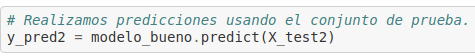
\includegraphics[width=0.5\textwidth]{imagenes/pred_lineal.png}
        \end{center}

        Comparamos los resultados de las predicciones con sus valores originales.
        \begin{center}
            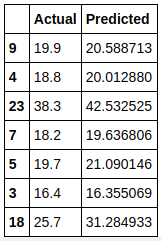
\includegraphics[width=0.2\textwidth]{imagenes/predicciones_lineal.png}
        \end{center}

        Para este modelo obtenemos un $MSE$ con valor de 
        $7.86$.
        \begin{center}
            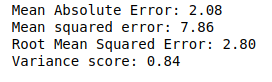
\includegraphics[width=0.4\textwidth]{./imagenes/MSE_Lineal.png}
        \end{center}

        % Ejercicio 7.b
        \item Comparando el MSE de este modelo con el del modelo anterior, 
        ¿cuál es menor? ¿a qué piensas que se debe?

        \textsc{Solución:} El menor valor de $MSE$ obtenido fue de $7.86$, 
        el cual corresponde al modelo creado usando regresión lineal. 

        Creo que en general ambos modelos pueden obtener un menor valor de 
        $MSE$ si el conjunto de datos fuera más grande, pues al ser muy 
        reducido, ambos no pueden \textit{aprender} lo suficiente como 
        para realizar predicciones muy buenas. Sin embargo, podemos notar 
        que el modelo creado usando regresión lineal es el que logró realizar 
        mejores predicciones (basándonos en las tablas creadas para comprar 
        los valores), pues los valores de las predicciones no difieren mucho 
        con respecto a los valores originales.
    \end{enumerate}
\end{enumerate}
\end{document}
